%&pdflatex
\begin{figure}[htp]
    \centering
    \textbf{This is a beautiful figure title}\par\medskip
    % \hspace*{\fill}
    \begin{subfigure}[b]{.3\textwidth}
        \centering
        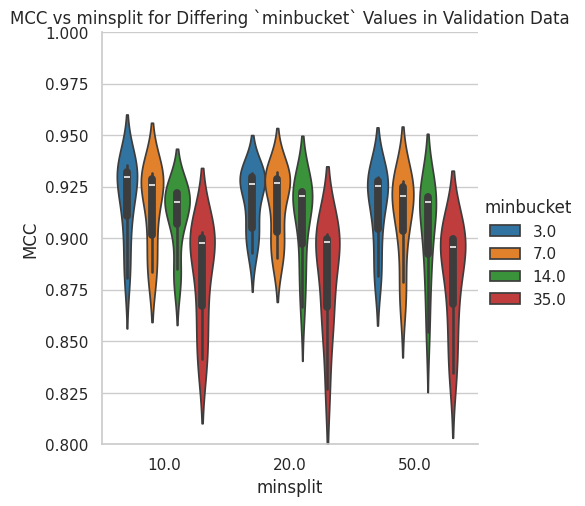
\includegraphics[scale=0.45]{cfgsl_mcc_minsplit_violin}
        \cprotect\caption{MCC versus \verb|minsplit| for varying values for \verb|minbucket|}
        \label{fig:cfgsl_mcc_minsplit_violin}
    \end{subfigure}
    \hfill
    \begin{subfigure}[b]{.3\textwidth}
        \centering
        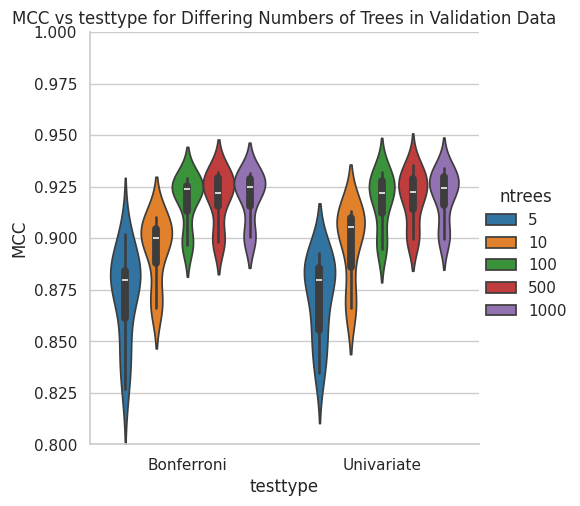
\includegraphics[scale=0.45]{cfgsl_mcc_testtype_violin}
        \cprotect\caption{MCC versus \verb|testtype| for varying numbers of trees.}
        \label{fig:cfgsl_mcc_testtype_violin}
    \end{subfigure}
    \hspace*{\fill}

    \begin{subfigure}[b]{.3\textwidth}
        \centering
        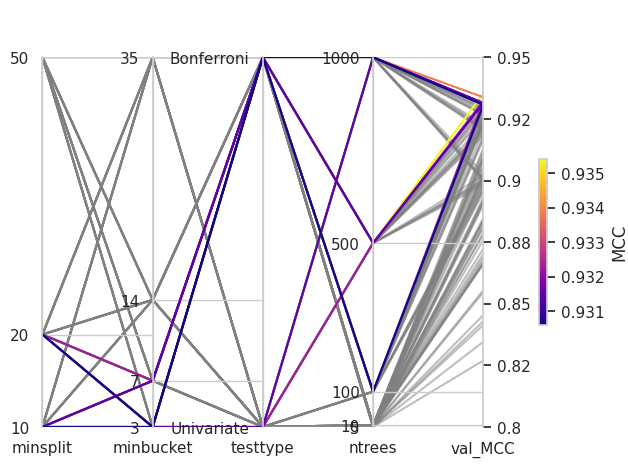
\includegraphics[scale=0.45]{cfgsl_pc}
        \caption{Top 10 forests by MCC}
        \label{fig:cfgsl_pc}
    \end{subfigure}
\caption{Results of gridsearch for the best hyperparameters for cforest.}
\end{figure}
